\section{РАЗРАБОТКА ПРОГРАММНЫХ МОДУЛЕЙ}
\label{sec:dev}

\subsection{Архитектура программного модуля}

Архитектура программного модуля для генерации и изменения 
изображений по текстовым описаниям объединяет две нейросети: одну для 
сегментации и выделения объектов на изображении, а другую – для 
применения диффузионной модели и создания новых изображений с учетом 
текстового описания необходимых изменений, данная архитектура 
представлена на рисунке~\ref{dev::shema}.

\begin{figure}[ht]
    \centering
    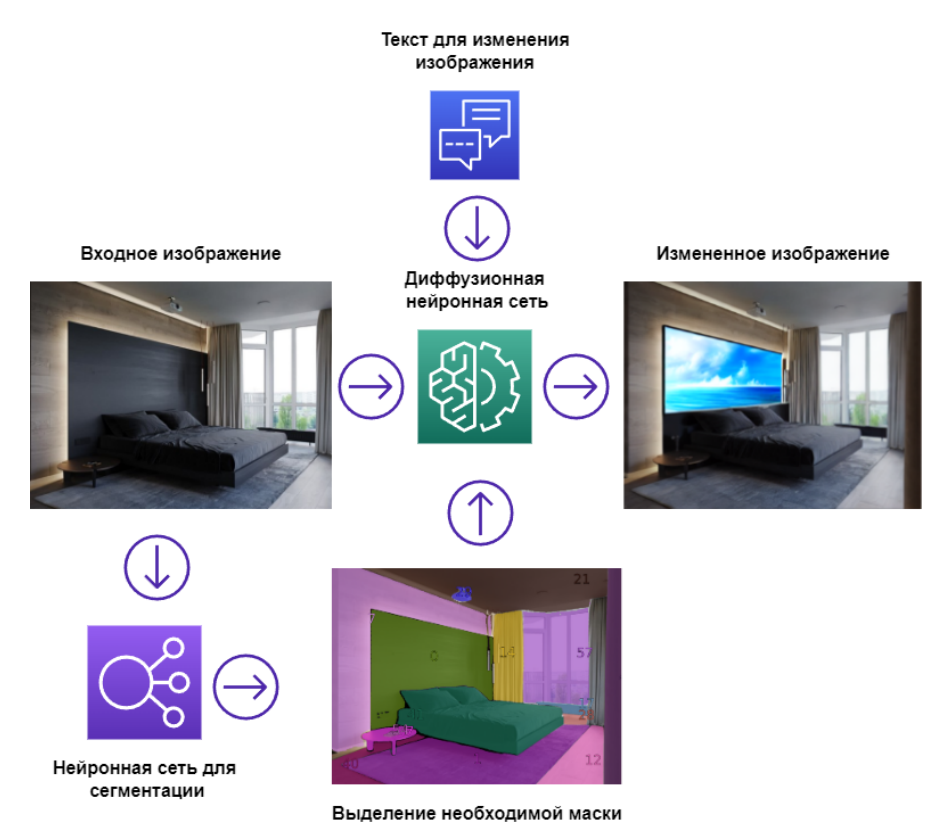
\includegraphics[width=0.7\linewidth]{module_shema.png}
    \caption{Упрощенная схема программного модуля для редактирования изображения с использованием текстовых описаний}
    \label{dev::shema}
\end{figure}

Архитектура программного модуля, разработанного для создания новых 
и измененных изображений на основе диффузионных моделей, состоит из 
нескольких этапов. В данном разделе мы подробно рассмотрим каждый этап 
процесса создания нового изображения и объясним, каким образом модуль 
выполняет свою функцию.

Перед началом работы модуля необходимо подготовить данные, 
которые будут использоваться для генерации нового изображения. Входные 
данные включают в себя изображение, которое будет служить основой для 
генерации.

Следующий этап – сегментация изображения (выбор маски). На этом 
этапе модуль использует первую нейросеть для сегментации изображения и 
выделения объектов, присутствующих на фотографии. Сеть анализирует 
изображение и генерирует маски, которые определяют области, 
соответствующие объектам, таким как стол, компьютер, цветок и другие 
элементы комнаты.

На последнем этапе, модуль использует диффузионную модель, для 
генерации нового изображения с учетом пользовательских запросов. 
Пользователь может предоставить текстовое описание желаемых изменений, 
например, запросить замену стола на диван. Для этого модуль обрабатывает 
текстовое описание и преобразует его в соответствующую маску, 
указывающую область, которую необходимо изменить. Затем диффузионная 
модель использует эту маску и исходное изображение, чтобы дорисовать или 
заменить объекты в указанной области в соответствии с запросом 
пользователя.

Итоговое изображение, полученное после работы диффузионной 
модели, представляет собой комбинацию исходного изображения и новых 
элементов, дорисованных в выбранной области.

\subsection{Подготовка данных}

Для того чтобы нейронная сеть могла обрабатывать изображение, оно 
должно быть представлено в виде числовых данных, которые сеть может 
анализировать и принимать решения на их основе. Обработка изображения 
включает в себя несколько шагов:

\begin{enumerate_step}
    \item Загрузка изображения. Сначала изображение должно быть загружено в память компьютера или сервера, где выполняется обработка. Обычно изображение представлено в формате, таком как JPEG или PNG, и может быть загружено из файловой системы или получено из других источников, например, с камеры или сети.
    \item Предварительная обработка. После загрузки изображения может потребоваться выполнить предварительную обработку для приведения его к определенному формату или размеру, а также для улучшения качества или нормализации данных. Некоторые типичные операции предварительной обработки включают изменение размера изображения, обрезку, поворот, нормализацию значений пикселей и прочие преобразования.
    \item Преобразование в числовой формат. Нейронные сети оперируют числовыми данными, поэтому изображение должно быть преобразовано в числовой формат, который сеть может понимать. Обычно изображение представляется в виде матрицы чисел, где каждый элемент матрицы соответствует значению яркости или цвета пикселя. Для цветных изображений часто используется формат RGB, в котором каждый пиксель представлен тройкой значений для красного, зеленого и синего цветовых каналов.
    \item Нормализация и стандартизация. После преобразования в числовой формат изображение может быть нормализовано и стандартизовано. Нормализация обычно выполняется для приведения значений пикселей в диапазон от 0 до 1 или от -1 до 1, чтобы упростить обучение и улучшить стабильность работы сети. Стандартизация может включать вычитание среднего значения и деление на стандартное отклонение, чтобы центрироватьданные и сделать их более сопоставимыми между разными изображениями.
    \item Подача изображения в нейронную сеть. После всех необходимых преобразований изображение может быть передано в нейронную сеть для обработки. Обычно это выполняется путем подачи изображения входным слоям сети, которые могут быть сверточными или полносвязными слоями. Значения пикселей изображения проходят через слои сети, где выполняются математические операции и применяются активационные функции для вычисления выходных значений сети.Таким образом, обработка изображения включает предварительную обработку, преобразование в числовой формат, нормализацию и стандартизацию, а затем подачу изображения в нейронную сеть для дальнейшей обработки и принятия решений.
\end{enumerate_step}

Таким образом, обработка изображения включает предварительную обработку, преобразование в числовой формат, нормализацию и стандартизацию, а затем подачу изображения в нейронную сеть для дальнейшей обработки и принятия решений.

\subsection{Сегментация изображений}

Сегментация изображений~-- это процесс выделения и разделения 
объектов на изображении путем создания соответствующих масок или 
сегментов, которые отображают границы и области объектов. В рамках 
данного проекта сегментация изображений играет важную роль в процессе
создания новых и измененных изображений по текстовым описаниям.

В программном модуле, после предварительной обработки входного 
изображения, оно передается в нейросеть, специально обученную для 
сегментации. Эта нейросеть анализирует изображение и создает маски, 
которые указывают области и границы объектов, найденных на фотографии. 
Каждая маска представляет собой матрицу пикселей, где значения пикселей в маске соответствуют принадлежности к определенному объекту.

В результате работы сети для сегментации мы получаем маски всех 
найденных объектов на изображении и их соответствующие границы. Эти 
маски используются в дальнейшем процессе, где пользователь может указать, 
какие изменения он хотел бы внести в определенные объекты на изображении.

Рассмотрим изображение представленное на рисунке~\ref{dev::dog}.

\begin{figure}[ht]
    \centering
    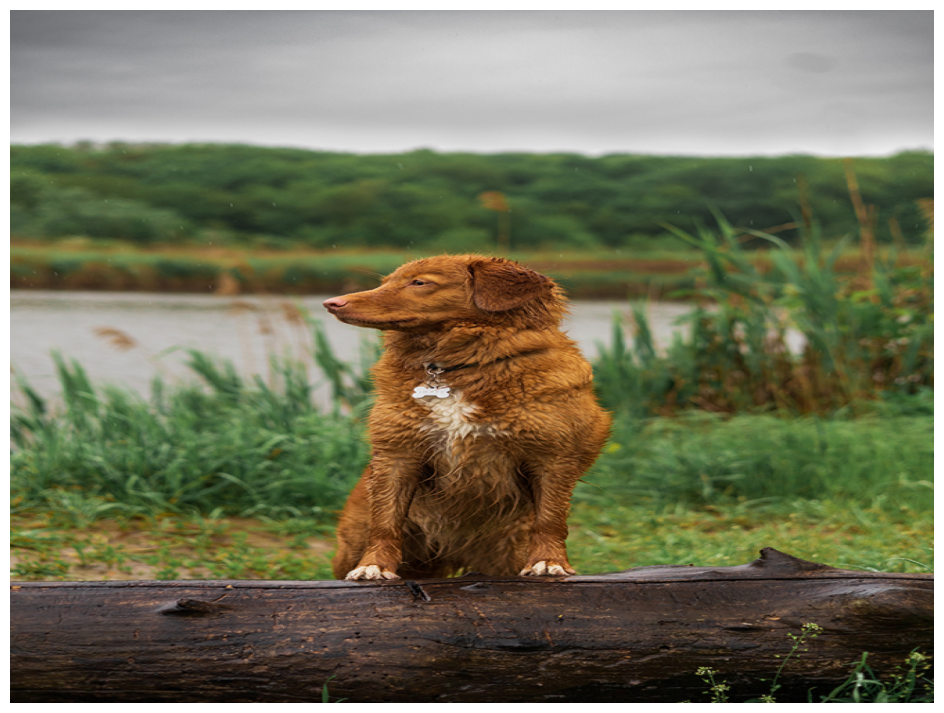
\includegraphics[width=.6\linewidth]{dog.png}
    \caption{Исходное изображение собаки}
    \label{dev::dog}
\end{figure}

Задача модели сегментации в данном случае: проанализировать всю 
фотографию и найти области, которые характерны для разных объектов. Для 
начала найдем все имеющиеся на изображении маски, результат работы 
сегментационный нейронной сети представлен на рисунке~\ref{dev::dog_all}.

\begin{figure}[ht]
    \centering
    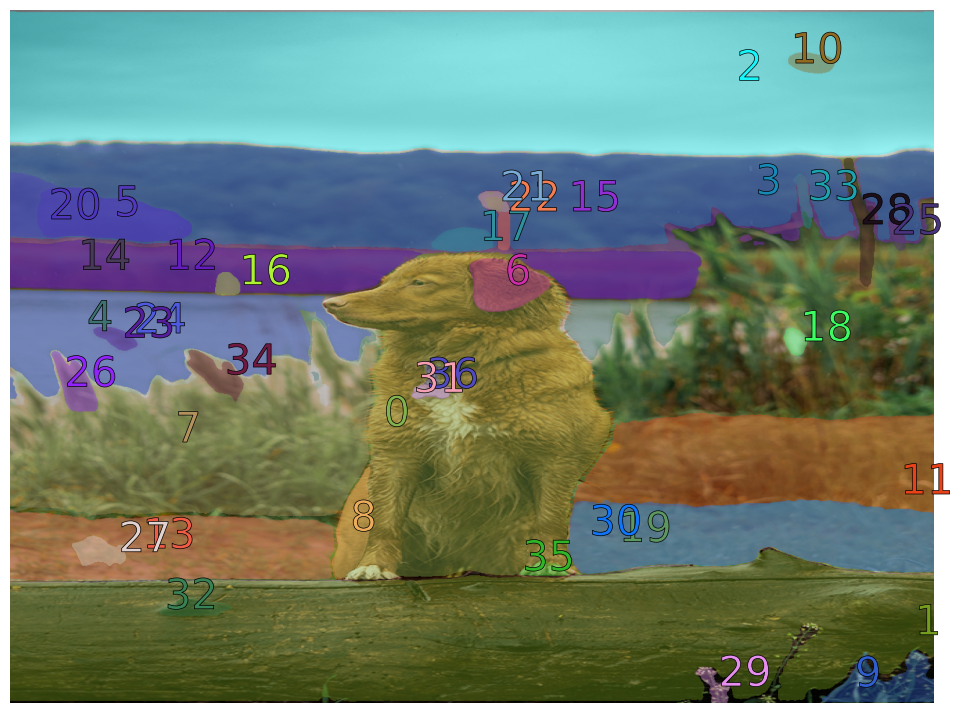
\includegraphics[width=.6\linewidth]{dog_all.png}
    \caption{Сегментированное изображение собаки}
    \label{dev::dog_all}
\end{figure}

Как можно увидеть нейронная сеть распознала гораздо больше объектов, 
чем можно рассмотреть на первый взгляд. Причем некоторые объекты состоят 
из других объектов, поэтому был разработан алгоритм, который среди всех 
масок объектов, находит основные, в которые входят более маленькие 
объекты. Этот алгоритм способен анализировать и организовать маски объектов, которые сгенерированы нейронной сетью. Он проходит через все маски, определяя основные из них. 

Эти основные маски содержат в себе один или несколько меньших объектов, что позволяет не только упростить общую картину распознавания, но и выделить ключевые элементы на изображении для дальнейшего анализа или обработки. Результат работы алгоритма для выделения основных объектов 
можно увидеть на рисунке~\ref{dev::dog_main}.

\begin{figure}[ht]
    \centering
    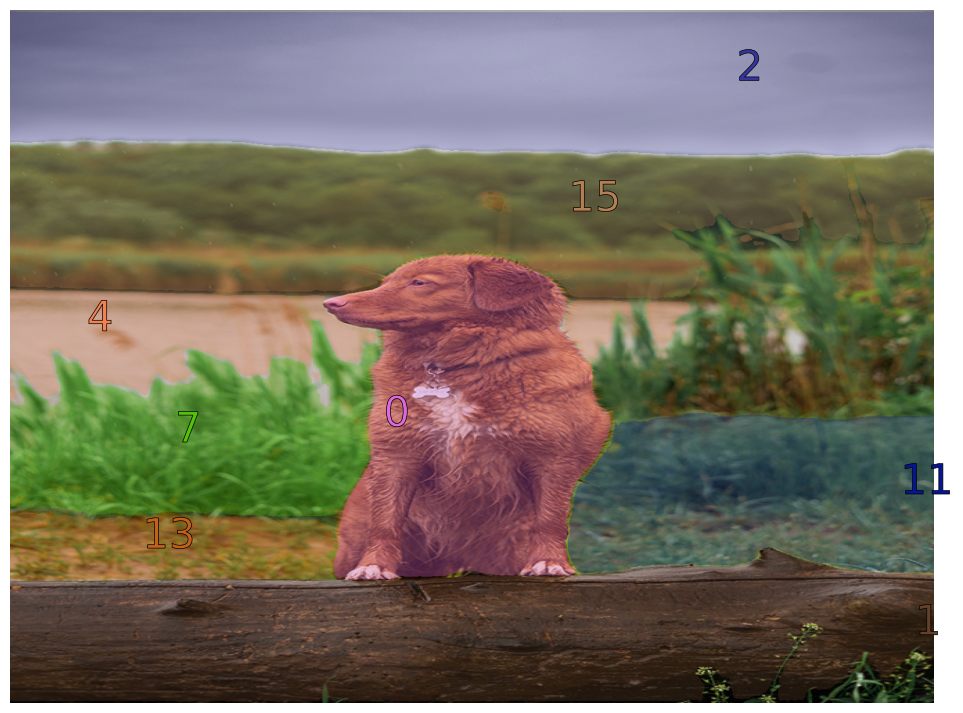
\includegraphics[width=.7\linewidth]{dog_main.png}
    \caption{Результат работы алгоритма для выделения главных масок на изображении}
    \label{dev::dog_main}
\end{figure}

Алгоритм работы функции автоматической сегментации:

\begin{enumerate_step}
    \item Начало.
    \item Получение пути к изображение \lstinline{image_path}.
    \item Сохранение пути в атрибуте \lstinline{self.image_path} объекта.
    \item Получение коррекцией размера \lstinline{image_resize}.
    \item Сохранение коррекцией размера в атрибуте \lstinline{self.image_resize}.
    \item Чтение изображения из пути \lstinline{self.image_path} с помощью функции \lstinline{cv2.imread}. По умолчанию OpenCV загружает изображения в формате BGR (Blue, Green, Red).
    \item Для корректной работы с цветами изображение конвертируется из формата BGR в RGB с помощью функции \lstinline{cv2.cvtColor}.
    \item Проверка на необходимость изменения размера. Если параметр \lstinline{self.image_resize} равен \lstinline{None} перейти к шагу~\ref{dev:1:cange_size}.
    \item Размеры изображения изменяются с использованием функции \lstinline{cv2.resize}, где \lstinline{resize[0]} и \lstinline{resize[1]} указывают новую ширину и высоту соответственно. Аргумент \lstinline{interpolation = cv2.INTER_AREA} выбран для лучшего качества при уменьшении размера.
    \item \label{dev:1:cange_size} Перемещение модели на GPU: Метод \lstinline{cuda()} вызывается для модели \lstinline{self.model}, что позволяет использовать графический процессор для ускорения вычислений при генерации масок.
    \item Инициализация генератора: Создаётся экземпляр \lstinline{mask_generator} класса \lstinline{SamAutomaticMaskGenerator}, который принимает обученную модель \lstinline{self.model} в качестве параметра. Этот объект будет использоваться для создания масок на изображении.
    \item Производство масок: Метод \lstinline{generate} объекта \lstinline{mask_generator} вызывается с параметром \lstinline{self.image} (изображение, загруженное и обработанное ранее). Метод возвращает список масок \lstinline{self.masks}, где каждая маска представляет собой область изображения, выделенную моделью.
    \item Цикл перебора масок.
    \item Присваивание уникального индекса для каждой маски в списке \lstinline{self.masks}.
    \item Конец цикла перебора списка масок.
    \item Создание списка \lstinline{res}, который будет использоваться для хранения результата. Каждый элемент этого списка будет кортежем, содержащим индекс маски и связанные с ней маски или пустой список. 
    \item Создание множества \lstinline{visited}, в которое добавляются индексы масок, уже учтенные в процессе обработки, чтобы избежать повторного анализа.
    \item Сортировка масок по убыванию площади. Это позволяет начать обработку с наибольших масок, которые могут включать в себя меньшие.
    \item \label{dev:1:outer_cicle} Цикл по маскам.
    \item Проверка находится ли текущая маска в visited. Если да то переход к следующему шагу цикла~\ref{dev:1:outer_cicle}.
    \item Создание пустого множества \lstinline{visited_inner_masks} для отслеживания уже проверенных масок в текущей итерации, чтобы избежать повторного сравнения.
    \item Создание пустого списка \lstinline{collected_inner_masks} для масок, которые находятся внутри текущей обрабатываемой маски и пересекаются с ней выше установленного порога.
    \item \label{dev:1:inner_cicle} Цикл по внутренним маскам.
    \item Проверка находится является ли текущая внутренняя маска текущей маской. Если да, то переход к следующему шагу цикла~\ref{dev:1:inner_cicle}.
    \item Проверка находится ли текущая внутренняя маска во множестве \lstinline{visited_inner_masks}. Если да то переход к следующему шагу цикла~\ref{dev:1:inner_cicle}.
    \item Создание переменной \lstinline{thres} , которая устанавливает порог для масок, позволяет контролировать чувствительность детекции объектов в анализируемых данных. Это значительно упрощает процесс сегментации.
    \item Проверка пересечения: Если сумма пересечений текущей и внутренней масок не превышает порог \lstinline{thres}, то переход к следующему шагу цикла~\ref{dev:1:inner_cicle}.
    \item Добавление текущей внутренней маски в \lstinline{collected_inner_masks}.
    \item Добавление индекса текущей внутренней маски в \lstinline{visited_inner_masks}.
    \item Добавление индекса текущей внутренней маски в \lstinline{visited}.
    \item Конец цикла по внутренним маскам.
    \item Если были найдены вложенные маски, в результат \lstinline{res} добавляется кортеж с индексом текущей маски.
    \item Индекс текущей маски добавляется в множество \lstinline{visited} после обработки всех вложенных масок.
    \item Конец цикла перебора масок.
    \item Возвращается список \lstinline{res}, содержащий данные о всех обработанных масках и их связях.
    \item Конец.
\end{enumerate_step}

\subsection{Определение связи между масками}

Этот алгоритм строит иерархию масок, определяя, какие маски содержат или перекрывают другие маски. Он анализирует набор масок, выявляя взаимосвязи между ними, и создает структуру данных, которая показывает, какие маски являются <<родительскими>> и какие <<дочерними>>.

\begin{enumerate_step}
    \item Начало.
    \item Получение набора масок \lstinline{masks}.
    \item Инициализация пустого списка который \lstinline{mask_list} для хранения масок.
    \item Приведение масок \lstinline{masks} к списку и присвоение его \lstinline{mask_list}.
    \item Инициализация пустого словаря \lstinline{mask_hierarchy}, который будет использоваться для хранения иерархии масок, где ключ~-- индекс маски-родителя, а значение~-- список масок-детей.
    \item \label{dev:2:main_cycle} Содержатся ли в \lstinline{mask_list} ещё элементы, если нет, то переход к шагу~\ref{dev:2:end}.
    \item Извлечение из начала списка \lstinline{mask_list} первая маска \lstinline{current_mask} для анализа.
    \item Вычисление размера маски \lstinline{current_mask_size}.
    \item Инициализация пустой переменной \lstinline{parent_mask} для хранения родительской маски. Эта переменная будет использоваться для хранения текущей маски-родителя для \lstinline{current_mask}.
    \item \label{dev:2:parent} Цикл поиска родительской маски.
    \item Вычисление размер маски \lstinline{mask_size}.
    \item Инициализация переменой \lstinline{intersection_size} для хранения размера пересечения между текущей маской и рассматриваемой.
    \item Вычисление пересечения между \lstinline{current_mask} и рассматриваемой маской.
    \item Вычисление размера пересечения \lstinline{intersection_size}.
    \item Вычисление размера пересечения с текущей родительской \lstinline{curr_intersection_size}.
    \item Если \lstinline{intersection_size} равен нулю нуля, то переход к следующей итерации цикла в шаге~\ref{dev:2:parent}.
    \item Если \lstinline{parent_mask} определен, либо текущее пересечение меньше, чем пересечение \lstinline{current_mask} с текущим то переход к следующей итерации цикла в шаге~\ref{dev:2:parent}.
    \item Обновление \lstinline{parent_mask} обновляется на текущую маску \lstinline{current_mask}.
    \item Установка индекса \lstinline{parent_mask_index} на индекс текущей маски в \lstinline{mask_list}.
    \item Конец цикла поиска родительской маски.
    \item Если \lstinline{parent_mask} найдена, то \lstinline{current_mask} добавляется в список детей \lstinline{parent_mask} в словаре \lstinline{mask_hierarchy}, используя \lstinline{parent_mask_index} как ключ.
    \item Если \lstinline{parent_mask} не найдена, то \lstinline{current_mask} добавляется в словарь с ключом, равным длине исходного списка \lstinline{masks}, что указывает на то, что у \lstinline{current_mask} нет родителя в списке.
    \item Переход к шагу~\ref{dev:2:main_cycle}.
    \item \label{dev:2:end} Возврат \lstinline{mask_hierarchy}: функция возвращает словарь \lstinline{mask_hierarchy}, который содержит все иерархические связи между масками.
    \item Конец.
\end{enumerate_step}

Этот алгоритм позволяет систематически определить отношения вложенности между масками, что может быть полезно в задачах анализа изображений для определения структурной сложности объектов на сцене.

\subsection{Алгоритм отображения масок на изображении}

Этот алгоритм позволяет визуализировать маски на изображении, каждую маскe выделяя уникальным цветом и помечая индексом, что упрощает идентификацию и анализ различных областей изображения.

\begin{enumerate_step}
    \item Начало.
    \item Получение списка масок \lstinline{anns}.
    \item Проверка, пустой ли список аннотаций anns. Если список пуст переход к шагу~\ref{dev:3:end}.
    \item Получение текущего осей графика: c помощью функции \lstinline{plt.gca()} извлекаются оси графика и сохраняются в переменной \lstinline{ax}.
    \item Отключение автомасштабирования: для осей графика устанавливается свойство \lstinline{set_autoscale_on(False)}, что предотвращает автоматическое масштабирование графика при добавлении новых элементов.
    \item Цикл по маскам.
    \item Инициализация переменной \lstinline{mask} для хранения текущей маски.
    \item Извлекается текущая маска, и она присваивается переменной \lstinline{mask}.
    \item Используется функция \lstinline{np.where(m)}, которая определяет индексы пикселей, соответствующие маски.
    \item Вычисление центральной точки маски для размещения текста с индексом маски. Координаты \lstinline{x_text} и \lstinline{y_text} вычисляются как медианные значения индексов по осям.
    \item Создание трёхканального белого изображение \lstinline{img} размером с маску.
    \item Генерация случайного цвета с помощью \lstinline{np.random.random((1, 3))}.
    \item Цикл применения цвета к каналам изображения.
    \item Применение цвета к каналу изображения.
    \item Конец цикла применения цвета к каналам изображения.
    \item Отображение изображения с маской \lstinline{ax.imshow(np.dstack((img, m)))} изображение с наложенной маской добавляется на график.
    \item Добавление текст с индексом маски \lstinline{ann_idx} с помощью \lstinline{ax.text}, размещаемый в центре маски с выбранным цветом и размером шрифта 30.
    \item Добавление тексту эффекта обводки с помощью \lstinline{path_effects.Stroke} для улучшения читаемости.
    \item Конец цикла по маскам.
    \item \label{dev:3:end} Конец.
\end{enumerate_step}

Пример работы алгоритма можно увидеть на рисунке~\ref{dev::masks}

\begin{figure}[ht]
    \centering
    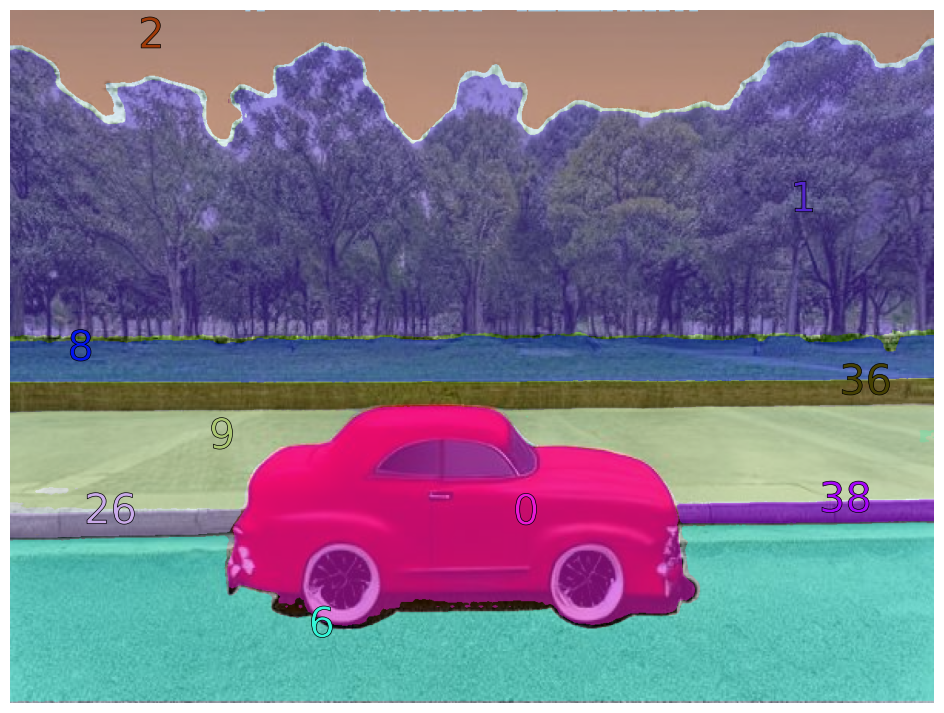
\includegraphics[width=0.95\linewidth]{car_main_masks.png}
    \caption{Выделение масок разными цветами и нумерация их}
    \label{dev::masks}
\end{figure}


\subsection{Генерация и редактирование изображений по текстовому описанию}

Процесс обработки и модификации изображений начинается с того, что в систему загружается исходное изображение. Затем оно подается на вход первой нейронной сети, задачей которой является сегментация. Этот шаг критически важен, поскольку он позволяет точно определить и выделить области на изображении, содержащие различные объекты. В процессе сегментации нейронная сеть анализирует изображение, чтобы создать маски пикселей для каждого идентифицированного объекта. Эти маски представляют собой выделенные области, которые точно соответствуют контурам и формам каждого объекта, что позволяет дальнейшему программному обеспечению более эффективно обрабатывать и анализировать каждый элемент изображения отдельно. 

Затем пользователь предоставляет текстовое описание изменений, 
которые требуется внести в выбранную маску объекта. Например, 
пользователь может указать, что хочет заменить задний фон на изображении. 
Текстовое описание передается второй нейронной сети, которая на основе 
маски объекта и текстовой информации генерирует новый объект, 
соответствующий описанию пользователя.
Применение диффузионных моделей позволяет плавно и естественно 
интегрировать новый объект в изначальное изображение, сохраняя его структуру и стиль. Этот метод обеспечивает сглаживание переходов между 
новым объектом и окружающими элементами, создавая единое и гармоничное 
изображение.
Для примера из всех масок, представленных на рисунке~\ref{dev::dog_main}, выберем 
маску под номером 2, на который изображен небо и попробуем с 
помощью диффузионной модели изменить вид на футуристический космос. 

Соответствующая маска представлена на рисунке~\ref{dev::dog_sky}.

\begin{figure}[ht]
    \centering
    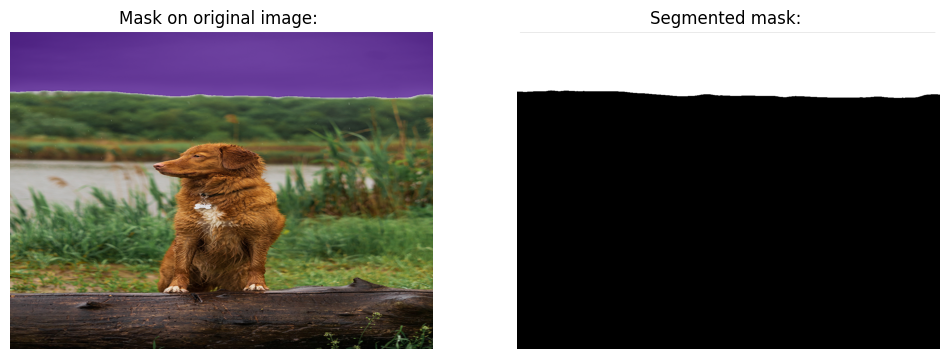
\includegraphics[width=1\linewidth]{dog_sky.png}
    \caption{Соответствующая маска неба на изображении с собакой}
    \label{dev::dog_sky}
\end{figure}

Далее на вход второй нейронной сети подадим данную маску, исходное 
изображение, а также текстовое описание необходимых изменений. Для 
примера попробуем изменить вид из окна на красивый вид с морем на фоне, 
текстовое описание: <<Space sky from the Earth realistic, high-resolution>>, где последнeе слово задает стилистику изображения. Результат работы диффузионной модели представлен на рисунке~\ref{dev::dog_sky_back}.

\begin{figure}[ht]
    \centering
    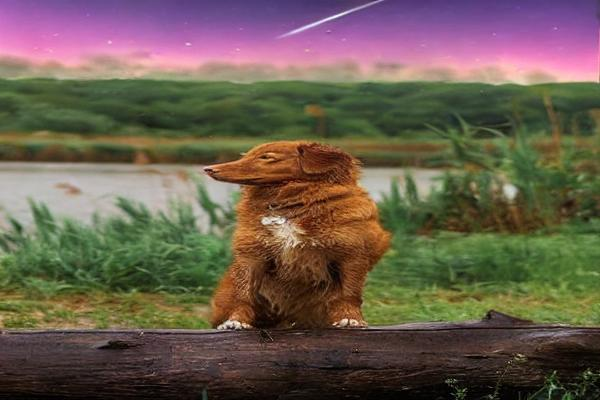
\includegraphics[width=.8\linewidth]{dog_sky_back.png}
    \caption{Измененное изображение с помощью текстового описания}
    \label{dev::dog_sky_back}
\end{figure}

Таким образом, архитектура программного модуля включает две нейронные сети, которые сотрудничают для генерации и редактирования изображений по текстовым описаниям. Этот подход позволяет пользователям легко вносить изменения в изображения, просто описывая желаемые модификации, а программный модель автоматически преобразует эти описания в новые объекты и интегрирует их в изначальное изображение с помощью диффузионной модели.

\subsection{Алгоритм графического интерфейса}

Этот алгоритм включает создание пользовательского интерфейса для
рисования маски на изображении в браузере и взаимодействие пользователя для задания стилевых предпочтений. После завершения пользовательского ввода, информация о маске и текстовый запрос собираются для дальнейшей обработки.

\begin{enumerate_step}
    \item Начало.
    \item Создается элемент \lstinline{div}, который будет использоваться как контейнер для всех интерактивных элементов интерфейса. Это базовый блок, в котором размещаются все остальные элементы управления.
    \item В контейнер \lstinline{div} добавляется параграф с текстом <<Размер кисти:>>, который служит описанием для последующего элемента управления~-- ползунка.
    \item Добавление элемента \lstinline{input} с типом \lstinline{range} (ползунок), который позволяет пользователю выбрать размер кисти для рисования. Этот элемент имеет минимальное значение 1, максимальное 100 и начальное установленное значение 40. Это дает пользователю гибкость в выборе толщины линии, которой он будет рисовать маску на изображении.
    \item Создание кнопки с текстом <<Поехали>>, которая будет использоваться для начала процесса рисования маски. Эта кнопка становится активной, когда пользователь готов начать рисование, и ее нажатие запускает процесс захвата рисунка маски.
    \item Добавление текстового поля, в котором пользователь может описать, что он хочет видеть на изображении после обработки. Это поле позволяет собрать текстовые данные для формирования текстового запроса, который будет использоваться в диффузионном процессе.
    \item Добавление в заголовок документа стилей CSS для всех элементов интерфейса, включая текстовые поля, кнопки, канвас и разделительные линии. Это включает стилизацию фона, рамок, размеров, а также интерактивные эффекты при наведении и фокусировке. Стилизация улучшает визуальное восприятие и удобство использования интерфейса.
    \item Создание дополнительного текстового поля для ввода стилевых атрибутов, таких как <<реалистичный, высокое разрешение>>. Это поле позволяет пользователю указать дополнительные характеристики стиля, которые он хочет видеть в результатах обработки изображения.
    \item Создание двух канвасов: один для отображения загруженного изображения и другой для рисования маски. Канвас для рисования маски наложен поверх канваса с изображением, что позволяет пользователю рисовать непосредственно на изображении. Это обеспечивает визуальную обратную связь о том, где и какая маска будет применена.
    \item Регистрация событий \lstinline{mousemove}, \lstinline{mousedown}, и \lstinline{mouseup} на канвасе для маски. Эти события управляют процессом рисования: при нажатии кнопки мыши начинается рисование, при перемещении мыши рисуется маска, а при отпускании кнопки рисование прекращается. Это позволяет создавать непрерывные линии или точки на канвасе в зависимости от движений пользователя.
    \item По нажатию на кнопку <<Поехали>> собирается изображение с канваса маски в формате JPEG. Также собираются текстовые данные из обоих текстовых полей, формируя окончательный текстовый запрос для диффузии.
    \item Все созданные элементы интерфейса удаляются из документа, чтобы очистить рабочее пространство, и возвращаются данные: изображение маски и сформированный текстовый запрос.
    \item Конец.
\end{enumerate_step}

Этот алгоритм детально описывает процесс создания интерактивного интерфейса для ручного рисования маски на изображении, сбора текстовых данных и последующей подготовки данных для использования в диффузионной модели. Пользовательский интерфейс включает инструменты для точного рисования маски, такие как регулируемые кисти, инструменты выделения и стирания, а также функции масштабирования и панорамирования для работы с различными участками изображения. После того как пользователь завершит создание маски, алгоритм собирает текстовые данные, описывающие изображение и желаемые характеристики. Эти данные затем конвертируются в формат, подходящий для диффузионной модели, которая использует их для генерации или модификации изображений на основе заданных параметров. Таким образом, алгоритм обеспечивает плавный и интуитивно понятный процесс от пользовательского ввода до генерации конечного результата.
